\documentclass[../main/main.tex]{subfiles}

\newdate{date}{6}{12}{2019}


\begin{document}

\marginpar{ \textbf{Lecture 16.} \\  \displaydate{date}. \\ Compiled:  \today.}

\section{Cubic term and first transition}
Let us consider more general forms of the Landay free energy. For example, in the case in which the symmetry is not violated, one can consider also odd temrs such as the cubic one.  In fact, we want to eneralize to include multicritical points, or phase transitions. The phase transitions can be obtained by introducing a cubic term in the Landau expansion. Remember that in the Ising model we have phase transition derived by symmetry breaking. Now, we have another type of phase transition.

The simplest Landau free energy that depends on a particular field is:
\begin{equation}
  \mathcal{L} ( \eta ,t,h)= a t \eta ^2 - w \eta ^3 + \frac{b}{4} \eta ^4 - h \eta
\end{equation}
where \( t \equiv \frac{T-T^*}{2} \) and \( w \) is an additional parameter that we fix to be positive, \( w>0 \).
\begin{remark}
For \( w<0 \) the results are the same, but in the \( \eta <0 \) diagram.
\end{remark}
To satisfy thermodynamic stability we require \( b>0 \), while
\begin{equation}
  a t = \frac{a}{2} ( T - T^*) \quad \text{if } \begin{cases}
    > 0 & T > T^* \\
    <0 & T < T^*
\end{cases}
\end{equation}
The equation of state for \( h \neq 0 \) is:
\begin{equation}
  \pdv{\mathcal{L}_G}{\eta } = 0 \quad \Rightarrow h = 2 a t \eta - 3 w \eta ^2 + b \eta ^3
\end{equation}
Let us consider the equilibrium states when \( h=0 \):
\begin{equation}
  h = 0 \quad \Rightarrow 0 = \eta ( 2 a t - 3 w \eta  + \beta \eta ^2)
\end{equation}
 The possible solutions are
\begin{equation}
  \begin{cases}
   \bar{\eta } = 0 & \text{disordered phase}\\
  \bar{\eta } = \frac{1}{4b} \qty(3w \pm \sqrt{q w^2 - 16 abt} ) & \text{ordered phases}
  \end{cases}
\end{equation}
Let us rewrite the 'ordered' solutions as
\begin{equation}
  \bar{\eta }_{\pm} = c \pm \sqrt{c^2 - \frac{at}{b}}
\end{equation}
where
\begin{equation}
  c = \frac{3w}{4b}
\end{equation}
Note that
\begin{equation}
  \bar{\eta }_{\pm} \in \R \iff c^2 > \frac{at}{b} \quad \Rightarrow \frac{T-T^*}{2} < \frac{c^2 b}{a} \equiv t^{**} \equiv  \frac{T^{**}-T^*}{2}
\end{equation}
It implies:
\begin{equation}
  T^{**} = T^* + \frac{2c^2b}{a}
\end{equation}
\begin{itemize}
\item If \( t> t^{**} \) \( (\iff T > T^ {**}) \), we have  \( \bar{\eta }_\pm \notin \R  \). The only real solution is \( \bar{\eta }=0  \) that is also the absolute minimum of \( \mathcal{L} \). The plot is shown in Figure \ref{fig:16_1}.
\begin{figure}[h!]
\centering
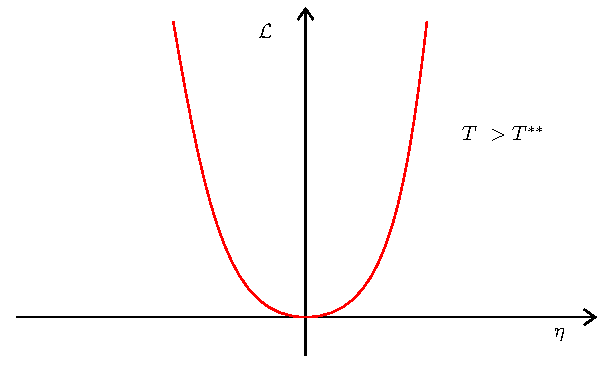
\includegraphics[width=0.6\textwidth]{../lessons/16_image/1.pdf}
\caption{\label{fig:16_1} Description.}
\end{figure}

\item If \( t \le t^{**} \) \( (\iff T \le T^ {**}) \), we have \( \bar{\eta }_\pm = c \pm \sqrt{c^2 - \frac{at}{b}} \in \R  \) are both possible solutions. One will be a local maximum and the other a local minimum.

\begin{itemize}
\item At \( T = T^{**}\), \( \bar{\eta }_- = \bar{\eta }_+   \) (flex point), as shown in Figure \ref{fig:16_2}.
\begin{figure}[h!]
\centering
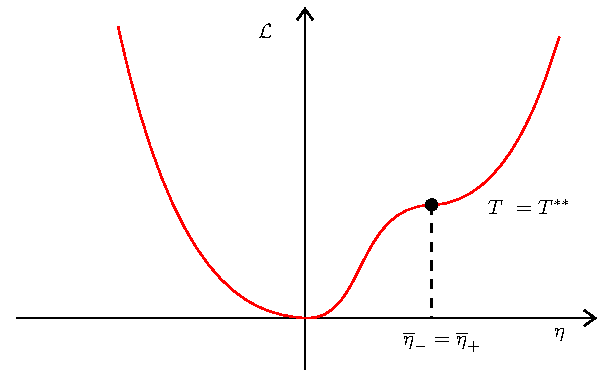
\includegraphics[width=0.6\textwidth]{../lessons/16_image/2.pdf}
\caption{\label{fig:16_2} Description.}
\end{figure}
\item For \( T_t < T < T^{**} \), \( \mathcal{L} (\bar{\eta }_+) >0  \). Since \( \mathcal{L} (\bar{\eta }=0 ) \), the solution \( \bar{\eta }_+  \) is a local minimum, as shown in Figure \ref{fig:16_3}.
\begin{figure}[h!]
\centering
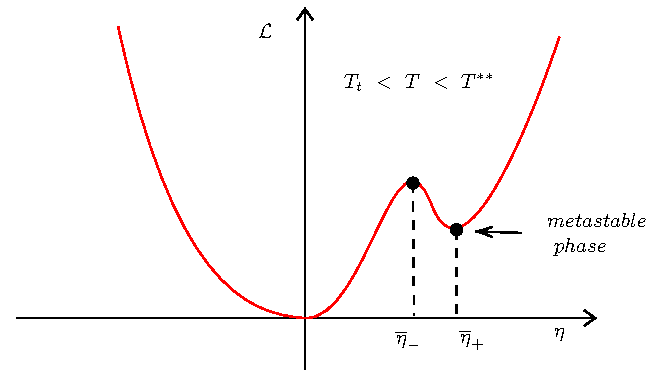
\includegraphics[width=0.6\textwidth]{../lessons/16_image/3.pdf}
\caption{\label{fig:16_3} Description.}
\end{figure}
\item By decreasing \( T \) firther one eventually reaches the value \( T=T_t \) at which the local minimum \( \mathcal{L} (\bar{\eta }_+ ) \) becomes zero, as in Figure \ref{fig:16_4}. \( T_t \)  is given by the coexistence condition
\begin{equation}
  \mathcal{L} (\bar{\eta }_+ ) = \mathcal{L} (0)
\end{equation}
that is the coexistence between the disordered and ordered phases!
\begin{figure}[h!]
\centering
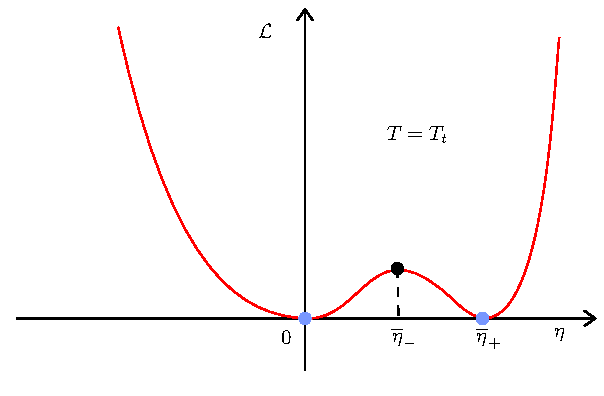
\includegraphics[width=0.6\textwidth]{../lessons/16_image/4.pdf}
\caption{\label{fig:16_4} Description.}
\end{figure}

In the plot of Figure \ref{fig:16_4} we see that there are two minima in the same line, this is  a first order transition.
At \( T=T_t \) the system undergoes a first order transition. To determine \( T_t \) we consider
\begin{equation}
  \begin{cases}
   \pdv{\mathcal{L}}{\eta } = 0 = \eta \qty(2 a t - 3 w \eta + 2 b \eta ^2)  & \text{extreme condition}\\
  \mathcal{L} ( 0 ) = \mathcal{L} ( \eta _+) & \text{coexistence condition}
  \end{cases}
\end{equation}
\begin{equation}
\Rightarrow
  \begin{cases}
   2 a t - 3 w \eta + 2 b \eta ^2 = 0\\
   a t - w \eta + \frac{b}{2} \eta ^2 = 0
  \end{cases}
\end{equation}
Solving with respect to \( \eta  \)  and \( t \) we get
\begin{equation}
  \begin{cases}
   \bar{\eta }_{+t} = + \frac{w}{b} >0 \\
    t_t = \frac{w^2}{2ba} \equiv \frac{1}{2} (T_t - T^*)
  \end{cases}
\end{equation}
\begin{equation}
  T_t = \frac{w^2}{b a} + T^*
\end{equation}
\begin{remark}
Note that \( T_t >T^* \).
\end{remark}
Since at \( T= T_t \) there is a first order transition does the system display latent heat?
\begin{equation}
  s = \eval{- \pdv{\mathcal{L}}{T} }_{\eta _t} = - \frac{1}{2} a \bar{\eta }_t^2 = - \frac{a}{2} \qty(\frac{w}{b})^2
\end{equation}
\begin{remark}
There is an entropy jump.
\end{remark}
The latent heat adsorbed to go from the ordered to the disordred phase is
\begin{equation}
  q = - T_t s = \frac{a}{2} T_t \qty(\frac{w}{b})^2
\end{equation}

\item Finally for \( T^* < T < T_t \), \( \eta = \bar{\eta }_+  \) becomes the global minimum ordered phase is the only stable one (Figure \ref{fig:16_5}).
\begin{figure}[h!]
\centering
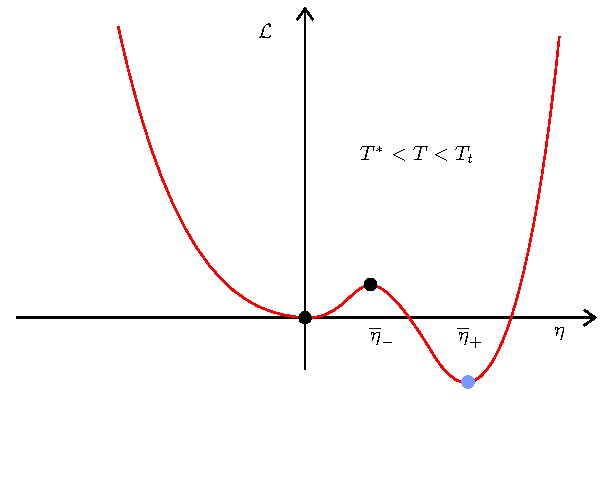
\includegraphics[width=0.6\textwidth]{../lessons/16_image/5.pdf}
\caption{\label{fig:16_5} Description.}
\end{figure}
\end{itemize}
\end{itemize}


\section{Phase stability and behaviour of \( \chi _T \equiv \pdv{\eta }{h}  \)}

Let us derive the equation of state with respect to \( h \)
\begin{equation}
  \pdv{}{h} \qty(\pdv{\mathcal{L}_G}{\eta } = 0 )   = \pdv{}{h} \qty(2 a t \eta - 3 w \eta ^2 + 2 b \eta ^3 = h)
\end{equation}
\begin{equation}
  \Rightarrow \chi \qty(2 a t - 6 w \eta + 6 b \eta ^2 ) =1
\end{equation}
The results is
\begin{equation}
  \chi _T = \frac{1}{2 a t - 6 w \eta + 6 b \eta ^2}
  \label{eq:16_1}
\end{equation}
We now make use of equation \eqref{eq:16_1} to compute the limit of stability of the phases we have found. 


\section{lesson}



Another possibility is studying multicritical point.
\begin{equation}
  \mathcal{L}_h (T, \Delta, \eta ) = \frac{a (t,\Delta )}{2} \eta ^2 + \frac{b(t,\Delta )}{4} \eta ^4 + c \eta ^6 - h \eta
\end{equation}
Consider \( \Delta  \) (\( \Delta _c \) is a critical value):
\begin{itemize}
\item \( \Delta < \Delta _c \): as \( T \) decreases, it will reach a value, we have \( a \) that decreases.
\begin{equation}
  T = T_c (\Delta ) \Rightarrow \begin{cases}
    a (T_c,\Delta ) = 0 \\
    b (T_c,\Delta ) > 0
\end{cases}
\end{equation}
\item \( \Delta > \Delta _c \): as \( T \) decreases, we will have \( a \) and \( b \) that will decrease too. At that point:
\begin{equation}
b (\bar{T},\Delta  ) = 0
\end{equation}
The free energy now is
\begin{equation}
  \mathcal{L} = \frac{a}{2} \eta ^2 + c \eta ^6
\end{equation}
The plot of the free energy is in figure 2. We have the coexistence of three lines.
\end{itemize}
Tricritical point:
\begin{equation}
  \Delta = \Delta _t, \quad T=T_t
\end{equation}
\begin{equation}
  a (\Delta _t, T_t) = b (\Delta _t, T_t) = 0
\end{equation}
\begin{equation}
  \mathcal{L}_t = c \eta ^6 - h \eta
\end{equation}


As we approach the critical point \( T \rightarrow T_c \), the correlation length
\( \xi \sim \abs{T-T_c}^{-\nu }  \) diverges.

Maybe mean field is not a very good approximation in proximity of the critical point. Question: how bad is the mean field approximation in proximity of the critical point?
\begin{equation}
  \expval{S_i S_j} \overset{MF}{\rightarrow } \expval{S_i} \expval{S_j}
\end{equation}
Calculate the error:
\begin{equation}
  E_{ij} = \frac{ \abs{\expval{S_i S_j}  - \expval{S_i} \expval{S_j}}   }{\expval{S_i}\expval{S_j}  }
\end{equation}
Define
\begin{equation}
  G_c (i,j) \equiv \expval{S_i S_j} - \expval{S_i} \expval{S_j} = \expval{(S_i -\expval{S_i} )(S_j - \expval{S_j} )}
\end{equation}
If we want to compute the error in the mean field, is always zero. So, if we want calculate the average with respect to fluctuations it does not work. We can either look at the variation in which the field is the internal one, or we can somehow try to make a variation not because of thermal fluctuations but because we control it. We do this by using an external field. This is the response theory with a variation of the field.

In order to do that, instead using an \( H \) we use an \( H_i \).
\begin{equation}
  Z = \Tr_{\{ S \} } \qty(e^{-\beta \qty(-J \sum_{\expval{ij} }^{} S_i S_j   - \sum_{i}^{} H_i S_i ) } )
\end{equation}
The definition of the thermal average is
\begin{equation}
  \expval{S_i} = \frac{\Tr_{\{ S \} } \qty(S_i e^{-\beta \qty(-J \sum_{\expval{ij} }^{} S_i S_j   - \sum_{i}^{} H_i S_i ) } ) }{Z}
  = \beta ^{-1} \pdv{\ln{Z} }{H_i} = - \pdv{F}{H_i}
\end{equation}
\begin{equation}
  \expval{S_i S_j} = \frac{\beta ^{-1}}{Z} \frac{\partial^2{Z} }{\partial{H_i} \partial{H_j}  }
\end{equation}
\begin{equation}
  G_c (i,j) = \beta ^{-1} \frac{\partial^2{\ln{Z} } }{\partial{H_i} \partial{H_j}  }
  = - \frac{\partial^2{F(\{ H_i \}  )} }{\partial{H_i} \partial{H_j}  }
\end{equation}
\begin{equation}
  \pdv{}{H_j} \expval{S_i} = \pdv{}{H_j} \qty[-\pdv{F}{H_i} ] = G_c (i,j)
\end{equation}
\begin{equation}
  M = \sum_{i}^{} \expval{S_i}
\end{equation}
\begin{equation}
  \pdv{M}{H_j} = \sum_{i}^{} \pdv{\expval{S_i} }{H_j} = \sum_{i}^{} G_c (i,j)
\end{equation}
\begin{equation}
  H_j = H_j (H)
\end{equation}
\begin{equation}
  \pdv{M}{H} = \sum_{j}^{} \pdv{M}{H_j} \pdv{H_j}{H}
  =  \beta \sum_{ij}^{} G_c (i,j)
\end{equation}
the last one is the susceptibility \( \chi _T \).
 Therefore,
 \begin{equation}
   \chi _T = \beta \sum_{i,j}^{} G_c (i,j)
 \end{equation}
 \begin{equation}
   G_c (i,j) \rightarrow G_c (\abs{i-j} ) \sim G (\abs{\va{r}} )
 \end{equation}
More or less, we want to compute the total relative error
\begin{equation}
  E_{TT} = \frac{\int_{V_ \xi }^{ } \dd[D]{\va{r}}  G_c (r)}{ \int_{V_ \xi }^{} \dd[D]{\va{r}} \eta ^2 } \ll 1
\end{equation}
This quantity is related to \( \chi _T \). Because of the fluctutations we can say that the quantity above is
\begin{equation}
  \sim  \frac{\beta ^{-1} \chi _T }{ \int_{V_ \xi }^{} \dd[D]{\va{r}} \eta ^2 }
\end{equation}
where \( \chi _T \sim t^{-\gamma  } \) and  the denominator it is \(  \sim t^{2 \beta } \xi ^D\).
\begin{equation}
  \frac{t^{-\gamma  }}{t^{2 \beta } t^{-\nu D}}
\end{equation}
\begin{equation}
  E \overset{t \rightarrow 0}{\sim } ^{-\gamma -2 \beta + \nu D } \ll 1
\end{equation}
\begin{equation}
  - \gamma - 2 \beta + \nu D \ge 0 \Rightarrow D > \frac{\gamma + 2 \beta  }{\nu }
\end{equation}
this is called the \emph{Ginzburg criterium}.

In the mean field we have: \( \gamma =1  \), \( \beta = 1/2 \). We obtain:
\begin{equation}
  D > \frac{2}{\nu }
\end{equation}
We have \( \nu _{MF} = 1/2 \). THerefore the dimension is \( D>4 \) for the mean field.
The
\begin{equation}
  D_c = \frac{\gamma + 2 \beta  }{2}
\end{equation}
is called \emph{upper critical dimension}.

Now we have a lower critical dimension (remember the last lessons!!) and an upper one.







\end{document}
